\documentclass[main.tex]{subfiles}

\begin{document}
\section{Данни и резултати}

Наличните бази данни за ЕЕГ са много по-малко от тези за реч. Това вероятно се дължи на факта, че съставянето им е доста по-трудно. Освен че изискват специална апаратура (тоест електроенцефалограф), изискванията към постановката са много по-строги. Тъй като се цели при записа да има възможно най-малко дразнители, освен представените от експеримента, трябва да се подсигури, че субектът е седнал удобно, на определено разстояние от монитора, не е болен, не му е студено или топло, не мига (или е със затворени очи), не говори и като цяло се движи възможно най-малко. Ако нещо в постановката се наруши, например човекът е мигнал, се трие целият запис. Често се подсигурява да не е бил консумиран кофеин (поне от страна на субекта, но вероятно е препоръчително и от страна на учения) в последните 24 часа и човекът да е имал нормален цикъл на съня. Допълнителна информация от типа дали субектът пуши, дали е левичар или десничар и какъв е по професия, се съобщава, тъй като не се знае дали не влияе на експеримента по някакъв начин. 

Целта на тази дипломна работа обаче е да се изследва комбинирането на сигнали от реч и ЕЕГ сигнали. Това изисква да имаме такава постановка, при която човекът говори, докато е свързан към електроенцефалограф, за да имаме данни от двата сигнала в един същи момент от време. Ако мигането е неприемливо, то комплексна дейност като говоренето е направо еретична за наличните бази данни. Разликата между ЕЕГ данни, извлечени докато субектът говори, и такива, при които субектът не говори, е много голяма, тъй като данните с намесена реч са много ``по-шумни''. Поради тази причина, и поради липсата\footnote{до колкото ни (или поне ``ми'') е известно} на подходяща база, такава трябваше да бъде създадена за конкретните цели.

Идеята е да се съчетаят най-често използваните похвати за създаване на емоционална речева база от една страна и емоциална ЕЕГ база от друга.

За реч най-често се използва една от следните две постановки: субектите (най-често актьори) четат предварително избрани емоционални изречения; субектите разказват емоционална случка по свой избор, например нещо преживяно или прочетено.

За ЕЕГ най-често се използва един от следните стимули: гледане на специално подбрани емоционални картинки\footnote{Например \url{https://web.archive.org/save/https://csea.phhp.ufl.edu/media/iapsmessage.html}}; слушане на специално подбрана емоционална музика; гледане на специално избрани емоционални клипчета.

Проблемът тук е, че за разлика от речевите бази данни, където не е нужно актьорите да изпитват емоцията, която изразяват, за да се отрази емоцията в ЕЕГ сигнала, емоцията трябва да е искрена. Тази задача е малко по-различна от задачата в стандартните ЕЕГ бази данни, защото тук изразяването на емоцията трябва да е по-продължително от времетраенето на картинка или клипче - трябва да бъде запазена докато субектът говори.

\begin{figure}[ht]%
    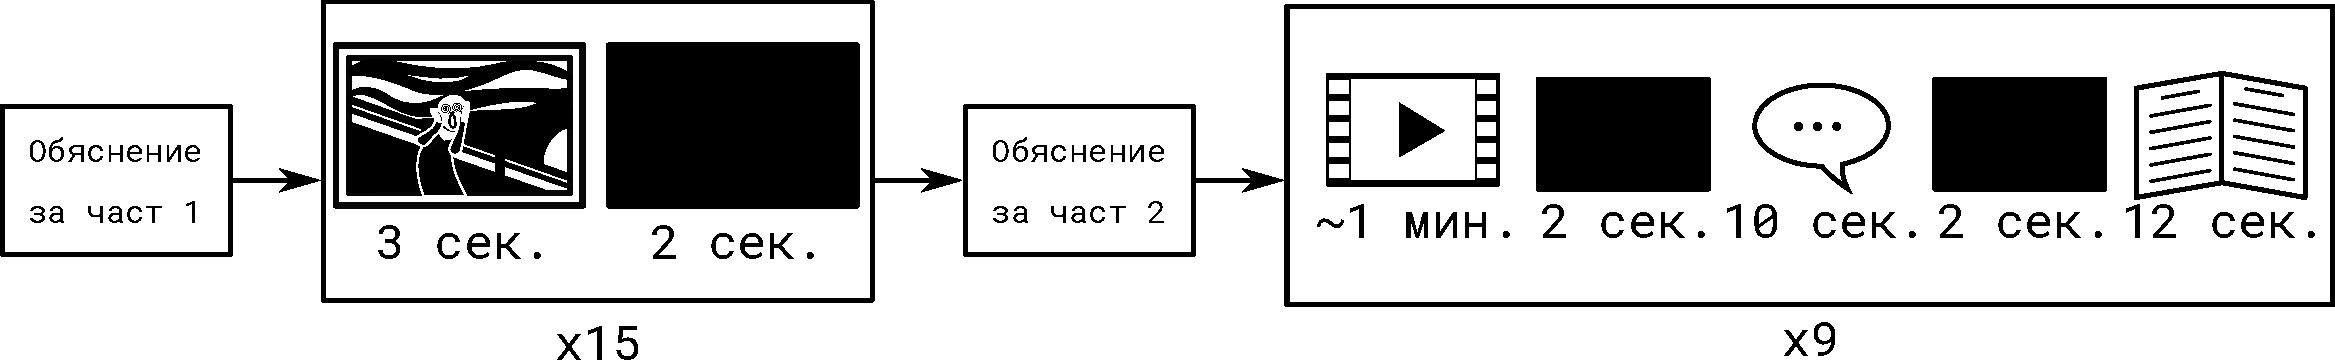
\includegraphics[width=\textwidth]{first_db}%
    \caption{}
    \label{fig:brain:res:1}
\end{figure}

Първият опит за емоционална база данни цели резултатът да е възможно най-близък до съществуващите вече ЕЕГ бази, но все пак да се съобразява с конкретните ни изискванията. Експериментът се състои от две части.
В първата част се гледат 15 специално избрани картинки (5 положителни, 5 отрицателни, 5 неутрални), като между картинките има пауза с черен екран. След това започва втората фаза, като първо на екрана се показва обяснение за протичането ѝ. Избира се едно от предварително подбраните емоционални клипчета (със средна дължина от една минута), субектът описва какво е видял на клипчето в продължение на десет секунди и след това чете показан на екрана текст за 12 секунди.
Клипчетата са 3 за щастие, 4 за тъга и 3 за гняв, като са подбрани от произволни източници (YouTube, сайтове за новини и телевизионни предавания) съгласно обратната връзка на въпроса "Какво те прави тъжен/ядосан/щастлив", зададен на около пет произволни човека. Текстовете, които субектът чете, са подбрани от прогнозата за времето, като се счита, че това ще произведе неутрални данни.
Субектът предварително знае постановката на опита и е помолен да ограничи движенията си максимално. Постановката е показана схематично на \autoref{fig:brain:res:1}, а информация за получените данни може да се види на \autoref{tab:brain:results:01}.

\begin{table}[h]
    \begin{center}
    \begin{tabular}{|l|r|r|} 
        \hline
        Емоция & Брой файлове & Обща дължина\\ 
        \hline
        Гняв & 3 & 0 мин. 30 сек.\\ 
        Щастие & 3 & 0 мин. 30 сек.\\ 
        Неутрално състояние & 10 & 2 мин. 00 сек. \\ 
        Тъга & 4 & 0 мин. 40 сек. \\ 
        \hline
    \end{tabular}
    \caption{Дължина и брой файлове от първия опит}
    \label{tab:brain:results:01}
    \end{center}
\end{table}

След експеримента първият и единствен субект сподели, че видеата не са успели да предизвикат искрена емоция. Това означава, че информацията за емоцията ще отсъства от ЕЕГ сигнала. Оказва се, че периодът от 1-2 минути, през който се гледа видео, е твърде кратък, за да може да се събуди непринудена емоционална реакция, ако видеата не са специално избрани с предварително знание за конкретния субект. Вероятно може да се постигне желаният ефект, ако гледаните видеа са достатъчно дълги, за да може субектът да развие емоционална привързаност, например с дължината на филм. За съжаление обаче, използването на мокри електроди позволява максимална продължителност на целия експеримент около 10-15 минути, след което време соленият разтвор по електродите изсъхва и съпротивлението им става твърде голямо, за да може да ги отчете уредът. Използването на картинки е безсмислено в конкретния случай, тъй като (се предполага че) събуждат емоция за части от секундата. Използването на музикални видеа изисква субектът да е чувствителен към музика. 

Всъщност съществува проблемът, че емоциите имат твърде различен характер и заради това се предизвикват и изразяват по различен начин. Щастието се предизвиква по-лесно от гнева чрез визуални стимули. Гневът обикновено изисква субектът да има лично отношение към темата, която му се представя, независимо от стимула. Щастието има много по-момента изява от тъгата, която се се изразява продължително, дори понякога в продължение на дни. Като цяло емоциите с ниска енергия се изразяват много по-трудно вербално от тези с висока. Но най-големият проблем идва, когато добавим и факта, че изглежда хората възприемат и изразяват емоцията по коренно различен начин един от друг.

Подобен тип проблеми често се разрешава със стратегия ``разделяй и владей'', затова естествено възниква въпросът дали може вместо да се намерят универсални за всички хора стимули, може да се намери разбиване на хората, спрямо начинът, по който се предизвиква емоция у тях (тяхната емоционална интелигентност). Подходяща е може би класификацията на Юнг, която цели да определи типа на характера. При нея всеки човек попада в една от 16 категории, в зависимост от това къде стои по четирите оси: интровертен-екстровертен, наблюдаващ-интуитивен,  чувстващ-мислещ, съдещ-приемащ\footnote{16 Personalities: Extraverted-Introverted, Sensing-Intuition, Thinking-Feeling,Judging-Peceiving}. Тоест дали ако двама човека попадат в една и съща категория, емоциите се предизвикват (и евентуално изразяват) по сходен начин. Класификацията на Юнг е избрана, тъй като има лесно-достъпни тестове, които ``определят'' класа. 
За целта петима участници са помолени да направят тест за класифициране на характери и след това да попълнят специално съставена съставена анкета. Тя цели да провери какъв тип стимул е нужен за предизвикването на всяка една от емоциите у участниците и да покаже евентуалната връзката с класификацията на Юнг.
Първо, за всяка една от изследваните емоции се търси най-подхдящият стимул, като възможностите са:
\begin{enumerate}
    \item Текст
    \item Видео
    \item Разговор
    \item Картинка
    \item Медията няма значение, само контекстът
\end{enumerate}
Участниците имат право да избират повече от един отговор.

Отговорите показват, че докато тъгата може да бъде предизвикана чрез пасивни методи като текст, щастието и гневът се предизвикват по-лесно в социална обстановка - чрез разговор. За съжаление се вижда, че няма пряка връзка между класификацията на Юнг и отговорите на анкетата. Това не означава, че попринцип този метод е неприложим, а само, че е нужен подходящ тест. Повечето признати в психологията тестове, обаче, изискват и професионално знание. 

Във втората част от анкетата резултатите стават още по-объркани. В нея участниците са помолени да изберат видео, картинка, текст или да опишат нещо, което ги предразполага емоционално за всяка една от емоциите. Оказва се, че предизвикването на емоция е твърде лично и няма засичащи се теми измежду всички отговори.

Последната част на анкетата не донесе допълнителен успех. В нея на участниците са представени стимули (видеа и картинки), за които трябва да бъде определена емоцията измежду неутрално състояние, щастие, тъга и гняв. Дори тук отговорите на участниците не съвпадат за повечето емоции.

От наличните данни не само се вижда, че хората, попадащи в един клас на Юнг, не споделят сходна чувствителност към стимулите, а че отговорите на всички участници генерално се различават. От една страна, ограничаването на възможните отговори за участниците би довело до по-голямо съвпадение на отговорите им, от друга, колкото повече трябва да променят отговорите си участниците, за да се вместят във формата, толкова по-принудена ще е и записаната емоция. Всъщност не е особено учудващо, че емоциите са толкова индивидуални. Според някои психолози (\cite{stupid-book}), емоциите изобщо не са универсални, а напротив - те са изцяло социална констуркция. Това означава, че ако участниците са от различен социален кръг (различна възраст, условия на живот, интереси), има малък шанс да имат сходен начин за изразяването на емоциите си. Ако обстановката и опитът формират емоцията у човек, то тогава комбинациите обстановка-човек-опит са почти уникални и съответно възприемането на емоция - индивидуално. В случая нито класическата, нито алтернативната теория дават обяснение как да се предизвика непринудена емоция в повече от един участник чрез честен експеримент.

Затова можем да направим по-малко честен опит, такъв, при който условията на експеримента зависят от самия субект, с цел да получим по-непринудена емоцията. С този замисъл е проведен вторият експеримент, при който емоцията се предизвиква от лични преживявания. От една страна, тъй като стимулът е избран от самия участник, не можем да гарантираме равни условия - тоесто субектите могат да изберат емоционално изживяване с различна интензивност. От друга, дори постановката на опита да е еднаква за всички, това не важи и за предизвиканата емоция. В някакъв смисъл, идеята е субектите да осигурят честността на експеримента, а не самата постановка на опита.

Вторият опит се отдалечава повече от стандартните постановки за ЕЕГ бази данни, тъй като използва множество различни дразнители, целящи да предразположи максимално участниците, според собствените им нужди. Дава се възможност на субектите сами да изберат видеа, които им действат емоционално, както и аудио запис, който да слушат по време на експеримента. Останалата част протича просто: субектът си избира емоция по свое желание и сам контролира включването на стимули. При натискане на бутон ``Enter'' се показва видео от предварително избраните, натискане на бутон ``Space'' означава съответно начало и край на аудио запис, по време на който субектът е свободен да говори каквото си избере. В експеримента няма минимален брой записи, които субектът трябва да направи, нито определена тема. След първите петнайсет минути, експериментът се прекъсва (ако е продължил толкова дълго), тъй като електродите изсъхват. Информация за получените данни е показана на \autoref{tab:brain:results:02}

\begin{table}[h]
    \begin{center}
    \begin{tabular}{|l|r|r|} 
        \hline
        Емоция & Брой файлове & Обща дължина\\ 
        \hline
        Гняв & 18 & 6 мин. 53 сек.\\ 
        Щастие & 0 & 0 мин. 00 сек. \\ 
        Неутрално състояние & 31 & 8 мин. 12 сек. \\ 
        Тъга & 45 & 15 мин. 13 сек. \\ 
        \hline
    \end{tabular}
    \caption{Дължина и брой файлове от втория опит}
    \label{tab:brain:results:02}
    \end{center}
\end{table}

При втората постановката е намесено много движение от страна на субекта, тъй като от него се изисква да натиска бутони. Начинът, по който протича експериментът за различните субекти, може да е напълно различен. Въпреки това, резултатите върху ЕЕГ данните значително се подобряват при данните от втория експеримент, което може да се обясни с липсата на искрена емоция при данните от първия експеримент. Тоест, независимо, че новите данни съдържат много повече шум, те съдържат и много полезна информация. 
Тъй като втората постановка не съдържа положителни данни, използваме тези от първия опит, за да можем да ги сравним. Резултатите са показани съответно на \autoref{tab:brain:results:03} и \autoref{tab:brain:results:04}. За пълнота, при класификацията само на речта от първия и втория експеримент се наблюдава средна класификационна точност от съответно $50.00\%$ и $75.56\%$. Това показва, че данните от първия опит сдържат по-малко полезна информация и в сигнала от реч, което вероятно се дължи на факта, че субектът нито е изпитал, нито е успял да изиграе емоцията добре.


\begin{table}[h]
    \begin{center}
    \begin{tabular}{|l|r r r r|} 
        \hline
        & Гняв & Щастие & Неутрално & Тъга \\ 
        \hline
        Гняв &  \textbf{33.33\%} & 0.00\% & 33.33\% & 33.33\% \\ 
        Щастие & 00.00\% & \textbf{100.00\%} & 0.00\% & 0.00\% \\ 
        Неутрално & 11.11\% & 0.00\% & \textbf{88.89\%} & 0.00\% \\ 
        Тъга & 0.00\% & 0.00\% & 100.00\% & \textbf{0.00\%}\\ 
        \hline
        \hline
        Общо & & & & \textbf{55.56\%}\\
        \hline
    \end{tabular}
    \caption{Матрица на грешките от първия опит}
    \label{tab:brain:results:03}
    \end{center}
\end{table}


\begin{table}[h]
    \begin{center}
    \begin{tabular}{|l|r r r r|} 
        \hline
        & Гняв & Щастие & Неутрално & Тъга \\ 
        \hline
        Гняв &  \textbf{100.00\%} & 0.00\% & 0.00\% & 0.00\% \\ 
        Щастие & 00.00\% & \textbf{100.00\%} & 0.00\% & 0.00\% \\ 
        Неутрално & 0.00\% & 0.00\% & \textbf{100.0\%} & 0.00\% \\ 
        Тъга & 0.00\% & 0.00\% & 4.44\% & \textbf{95.56\%}\\ 
        \hline
        \hline
        Общо & & & & \textbf{98.89\%}\\
        \hline
    \end{tabular}
    \caption{Матрица на грешките от втория опит}
    \label{tab:brain:results:04}
    \end{center}
\end{table}

Тъй като данните са малко, в следващия раздел ще обединим резултата от първия и втория експеримент. Матрицата на грешките при класификацията на ЕЕГ сигнала за обединените данни може да се види на \autoref{tab:brain:results:05}

\begin{table}[h]
    \begin{center}
    \begin{tabular}{|l|r r r r|} 
        \hline
        & Гняв & Щастие & Неутрално & Тъга \\ 
        \hline
        Гняв &  \textbf{80.33\%} & 5.00\% & 15.33\% & 0.00\% \\ 
        Щастие & 25.00\% & \textbf{75.00\%} & 0.00\% & 0.00\% \\ 
        Неутрално & 0.00\% & 2.50\% & \textbf{97.50\%} & 0.00\% \\ 
        Тъга & 0.00\% & 2.08\% & 10.42\% & \textbf{87.50\%}\\ 
        \hline
        \hline
        Общо & & & & \textbf{85.00\%}\\
        \hline
    \end{tabular}
    \caption{Матрица на грешките при комбиниране на данните от първия и втория опит}
    \label{tab:brain:results:05}
    \end{center}
\end{table}

\end{document}
